\section{Logo Entwürfe}
\begin{figure} [tp]
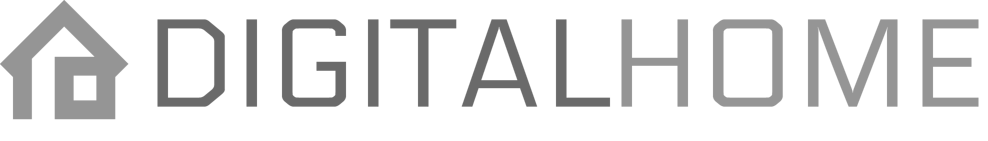
\includegraphics[width=\textwidth]{./img/logo1.png}
\caption{Der erste Logo Entwurf}
\label{logo1}
\end{figure}
\begin{figure} [tp]
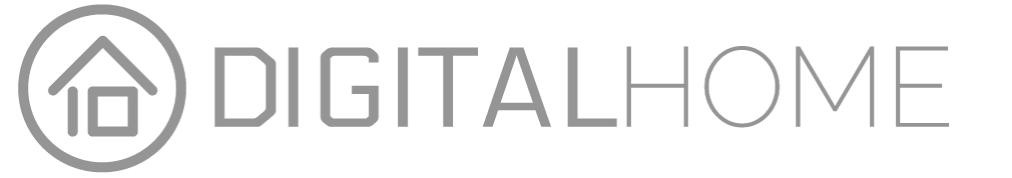
\includegraphics[width=\textwidth]{./img/logo2.png}
\caption{Der zweite Logo Entwurf}
\label{logo2}
\end{figure}
Nun muss für Digital Home ein Logo gefunden werden. Der erste Entwurf entstand im Zuge des minimalistischen sowie des zeitgemäßen Comps. Der zweite Logoentwurf entstand im Zuge des innovativen Comps. Um die Qualität des Logos besser beurteilen zu können, wurde hier das ARMM-Modell \footcite[vgl.][]{ARMM:model} sowie die Gestaltpsychologie \footcite[vgl.][]{gestalt} zu Rate gezogen. Auf Grund des ARMM-Modells (Attention, Response, Memory, Meaning) ist die Aufgabe des Digital-Home-Logos, die Digitalisierung des Hauses in einem einfachen Symbol festzuhalten, das Aufmerksamkeit erregt, eine passende Emotion hervorruft, gut zu merken ist und einen tieferen Sinn hat. Deshalb besteht das Logo aus einem abstrahierten Haus, dessen Fassade aus 1 und 0 besteht.

Aufmerksamkeit erregt das Logo durch das Haussymbol. Haussymbole suggerieren das „nach Hause“ gehen („Home“ bei Websites, „Startseite“ in Webbrowsern) und wirken damit sofort vertraut auf den Nutzer. Der Nutzer fühlt sich wohl und reagiert mit Vertrauen gegenüber der Brand "Digital Home". Da Menschen sich im wesentlichen Umrisse und simple Formen merken (Gesetz der Prägnanz \footcite[vgl.][]{gestalt}), wurde hier besonders auf Einfachheit des Logos, geringe Anzahl an visuellen Elementen geachtet. Dadurch wird auch die Bedeutungsdichte höher, da es in beiden Entwürfen zwei visuelle Objekte (Dach, Fassade) gegenüber zwei Bedeutungen gibt (Haus, Digitalisierung). Dieses 1:1-Verhältnis rechtfertigt die Elemente des Logos und zeigt, dass hier nicht unnötig viele Elemente ohne Hintergedanken verwendet wurden.

Der Schriftzug enthält den Font Electrolize, der technisch wirkt und daher für dieses Logo gut geeignet scheint. Auf Grund der Unifarbigkeit lassen sich die Logos auf jedem Hintergrund benutzen.


Die Entwürfe unterscheiden sich in der Umsetzung dieser Grundidee. Im ersten Entwurf (Abbildung \ref{logo1}) werden bewusst Ecken gezeigt, sie sollen dem Logo einen technisch seriösen Aspekt geben. Die geraden Linien wirken simpel und straight-forward. Das „Dach“ wurde bewusst mit der „Fassade“ verbunden, damit das Logo eine einheitliche Form bildet und damit als Einheit zu erkennen ist (Gesetz der Geschlossenheit \footcite[vgl.][]{gestalt}). Insgesamt wirkt das Logo sehr technisch und kantig.


Das zweite Logo (Abbildung \ref{logo2}) bietet runde Ecken, die das Logo runder und weicher erscheinen lassen. Dazu wird es durch einen Kreis eingerahmt, um das Logo einen festgelegten Platz zuzuweisen. Dabei wird darauf geachtet, dass das „Dach“ von der „Fassade“ des Hauses visuell getrennt ist, da sonst die „1 0“-Symbolik nicht mehr zum Vorschein kommt, ohne dass dabei die Zusammengehörigkeit der Objekte in Frage steht (Gesetz der Nähe \footcite[vgl.][]{gestalt}). Außerdem wird hier eine Pfeilform sichtbar. Pfeile zeigen, dass etwas in einer bestimmten Richtung geschieht (z.B. Bewegung). Deshalb werden Pfeile mit Bewegung assoziiert (z.B. Vektoren). Wichtig ist dabei, in welche Richtung der Pfeil zeigt. Man kennt Pfeile vor allem aus Diagrammen, und nimmt die Richtungen oben und rechts als positiv war, wobei ein Pfeil nach rechts eine Zeitveränderung suggeriert (z.B. fortlaufendes x bei Funktionen), während der Pfeil nach oben eher einen Wertzuwachs zeigt (z.B. Aktienkurse). Der Pfeil im Logo wertet das Logo dementsprechend auf und erhöht die bereits erwähnte Bedeutungsdichte.

\subsection{Fontwahl}
Für die Gestaltung des Schriftzuges gibt es hier zwei verschiedene Vorgehensweisen. Normalerweise werden Wörter durch Freiräume getrennt (Leerzeichen, Carriage Return). Dies ist hier jedoch nicht empfehlenswert, da eine Trennung der Wörter zur Bildung von zwei verschiedenen Elementen innerhalb des Logos führen würde. Es würde dann aus dem Trademark, dem Schriftzug und noch einem Schriftzug bestehen. Um das zu umgehen, werden die Wörter mit anderen visuellen Mitteln unterschieden. Aus Gründen der Lesbarkeit wird das Letterspacing nicht verändert.

Das erste Logo setzt auf eine einheitliche Schriftart und unterscheidet die Wörter „Digital“ und „Home“ durch verschiedene Farben. Dadurch entsteht ein Bruch mit der Idee der Unifarbigkeit, die einheitliche Font bringt jedoch Konsequenz in das Schriftbild des Logos.
Das zweite Logo bleibt unifarben und damit flexibel, während die Schrift sich ändert. Diese zweite Font ist „Raleway“, welche auch auf der Website verwendet wird. Trotz der Tatsache, dass es sich bei beiden Fonts um Sans-serif Typefaces handelt, lassen sich beide Wörter aufgrund der unterschiedlichen Font-weight gut erkennen. Das Logo bleibt farblich flexibel, während die dünne Raleway Font Modernität und Leichtigkeit vermittelt und sich mit der technischen Electrolize Font zur perfekten Repräsentation der Digital-Home-Marke vereint.
